\section{Umsetzung}

\subsection{Labor Netzwerk Architektur} \label{subsec:Labor-Netzwerk-Architektur}
Mit der zur Verfügung gestellten Hardware ist die folgende Netzwerk Architektur entstanden.

Folgende zentrale Überlegungen sind eingeflossen:

\begin{itemize}
	\item Campus Netzwerk mit mehreren Gebäuden, um das Wandern von Geräten zu simulieren.
	\item Mischung der zur Verfügung stehenden Switches (Catalyst 9300 \& 3850) in der Fabric Edge Nodes, um Verhalten zu vergleichen.
	\item Management Netzwerk ist inbound. Kabelführung zu jedem Switch ist meistens von den Gegebenheiten in typischen Gebäuden nicht möglich.
\end{itemize}


\begin{figure}[H]
	\centering
	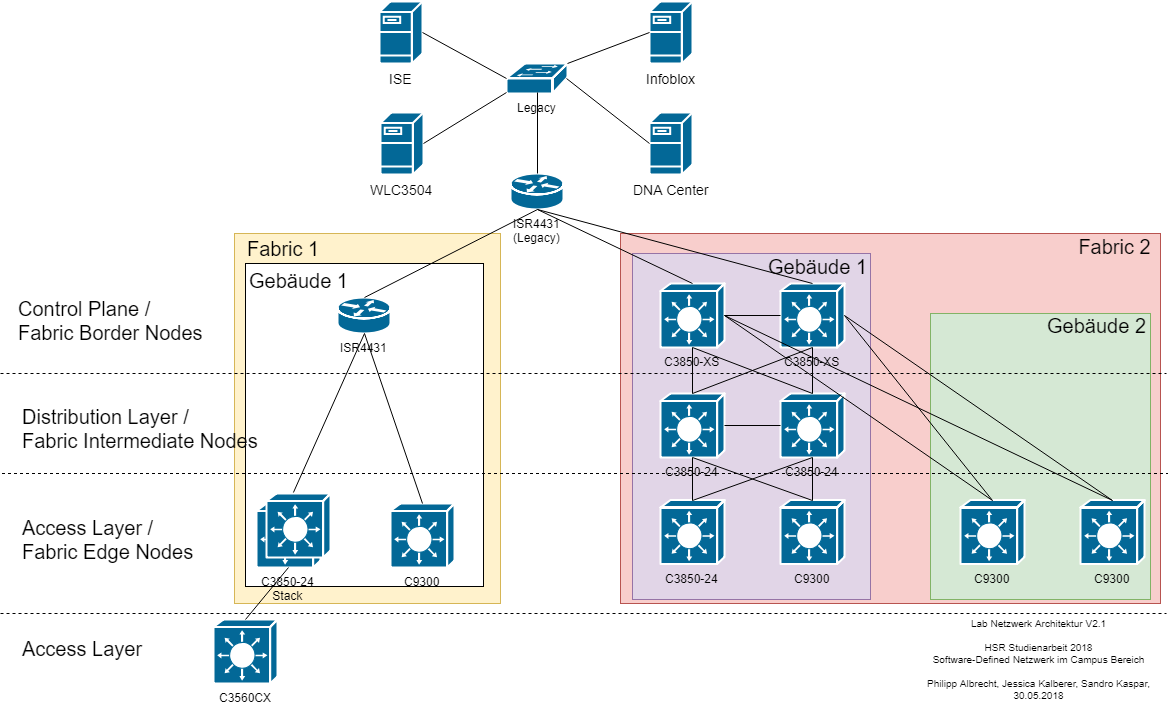
\includegraphics[width=1\linewidth]{img/LabNetworkArchitecture.png}\\[1px]
	\caption{SDN Netzwerk Architektur}
	\label{fig:LabNetworkArchitecture}
\end{figure}

Unsere Netzwerk Architektur besteht aus drei Layer. Weitere Informationen über die Funktion des Fabric Border, Fabric Intermediate und Fabric Edge sind im Kapitel der Technologien beschrieben (siehe Kapitel \ref{CampusFabric} Campus Fabric).

\subsubsection{Empfehlungen von Cisco}
Die ursprüngliche Architektur wurde an die Empfehlungen von Cisco angepasst. Die Border sind wie in der Abbildung oben ersichtlich nun Catalyst 3850 und die Catalyst 9300 kommen erst als Edge zum Zug, anstatt schon als Border.
\begin{figure}[H]
	\centering
	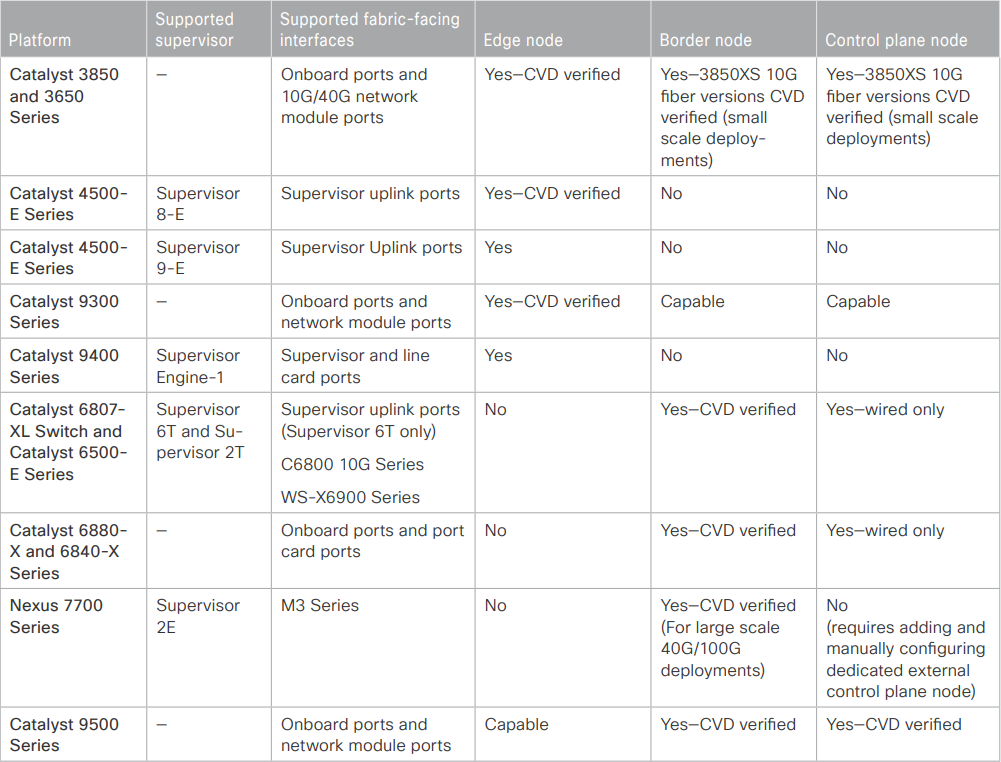
\includegraphics[width=1\linewidth]{img/SDA-switchingplatformanddeploymentcapabilities.png}\\[1px]
	\caption{SDA Switching Platform and Deployment Capabilities \cite{sda-designguide}}
	\label{fig:SDA Switching Platform and Deployment Capabilities}
\end{figure}

\subsection{Verkabelungsplan}
Auf nachfolgendem Verkabelungsplan sind die genauen Ports zwischen den Geräten ersichtlich, so dass für Konfigurationen die richtigen Interfaces schnell gefunden werden können.
\begin{figure}[H]
	\centering
	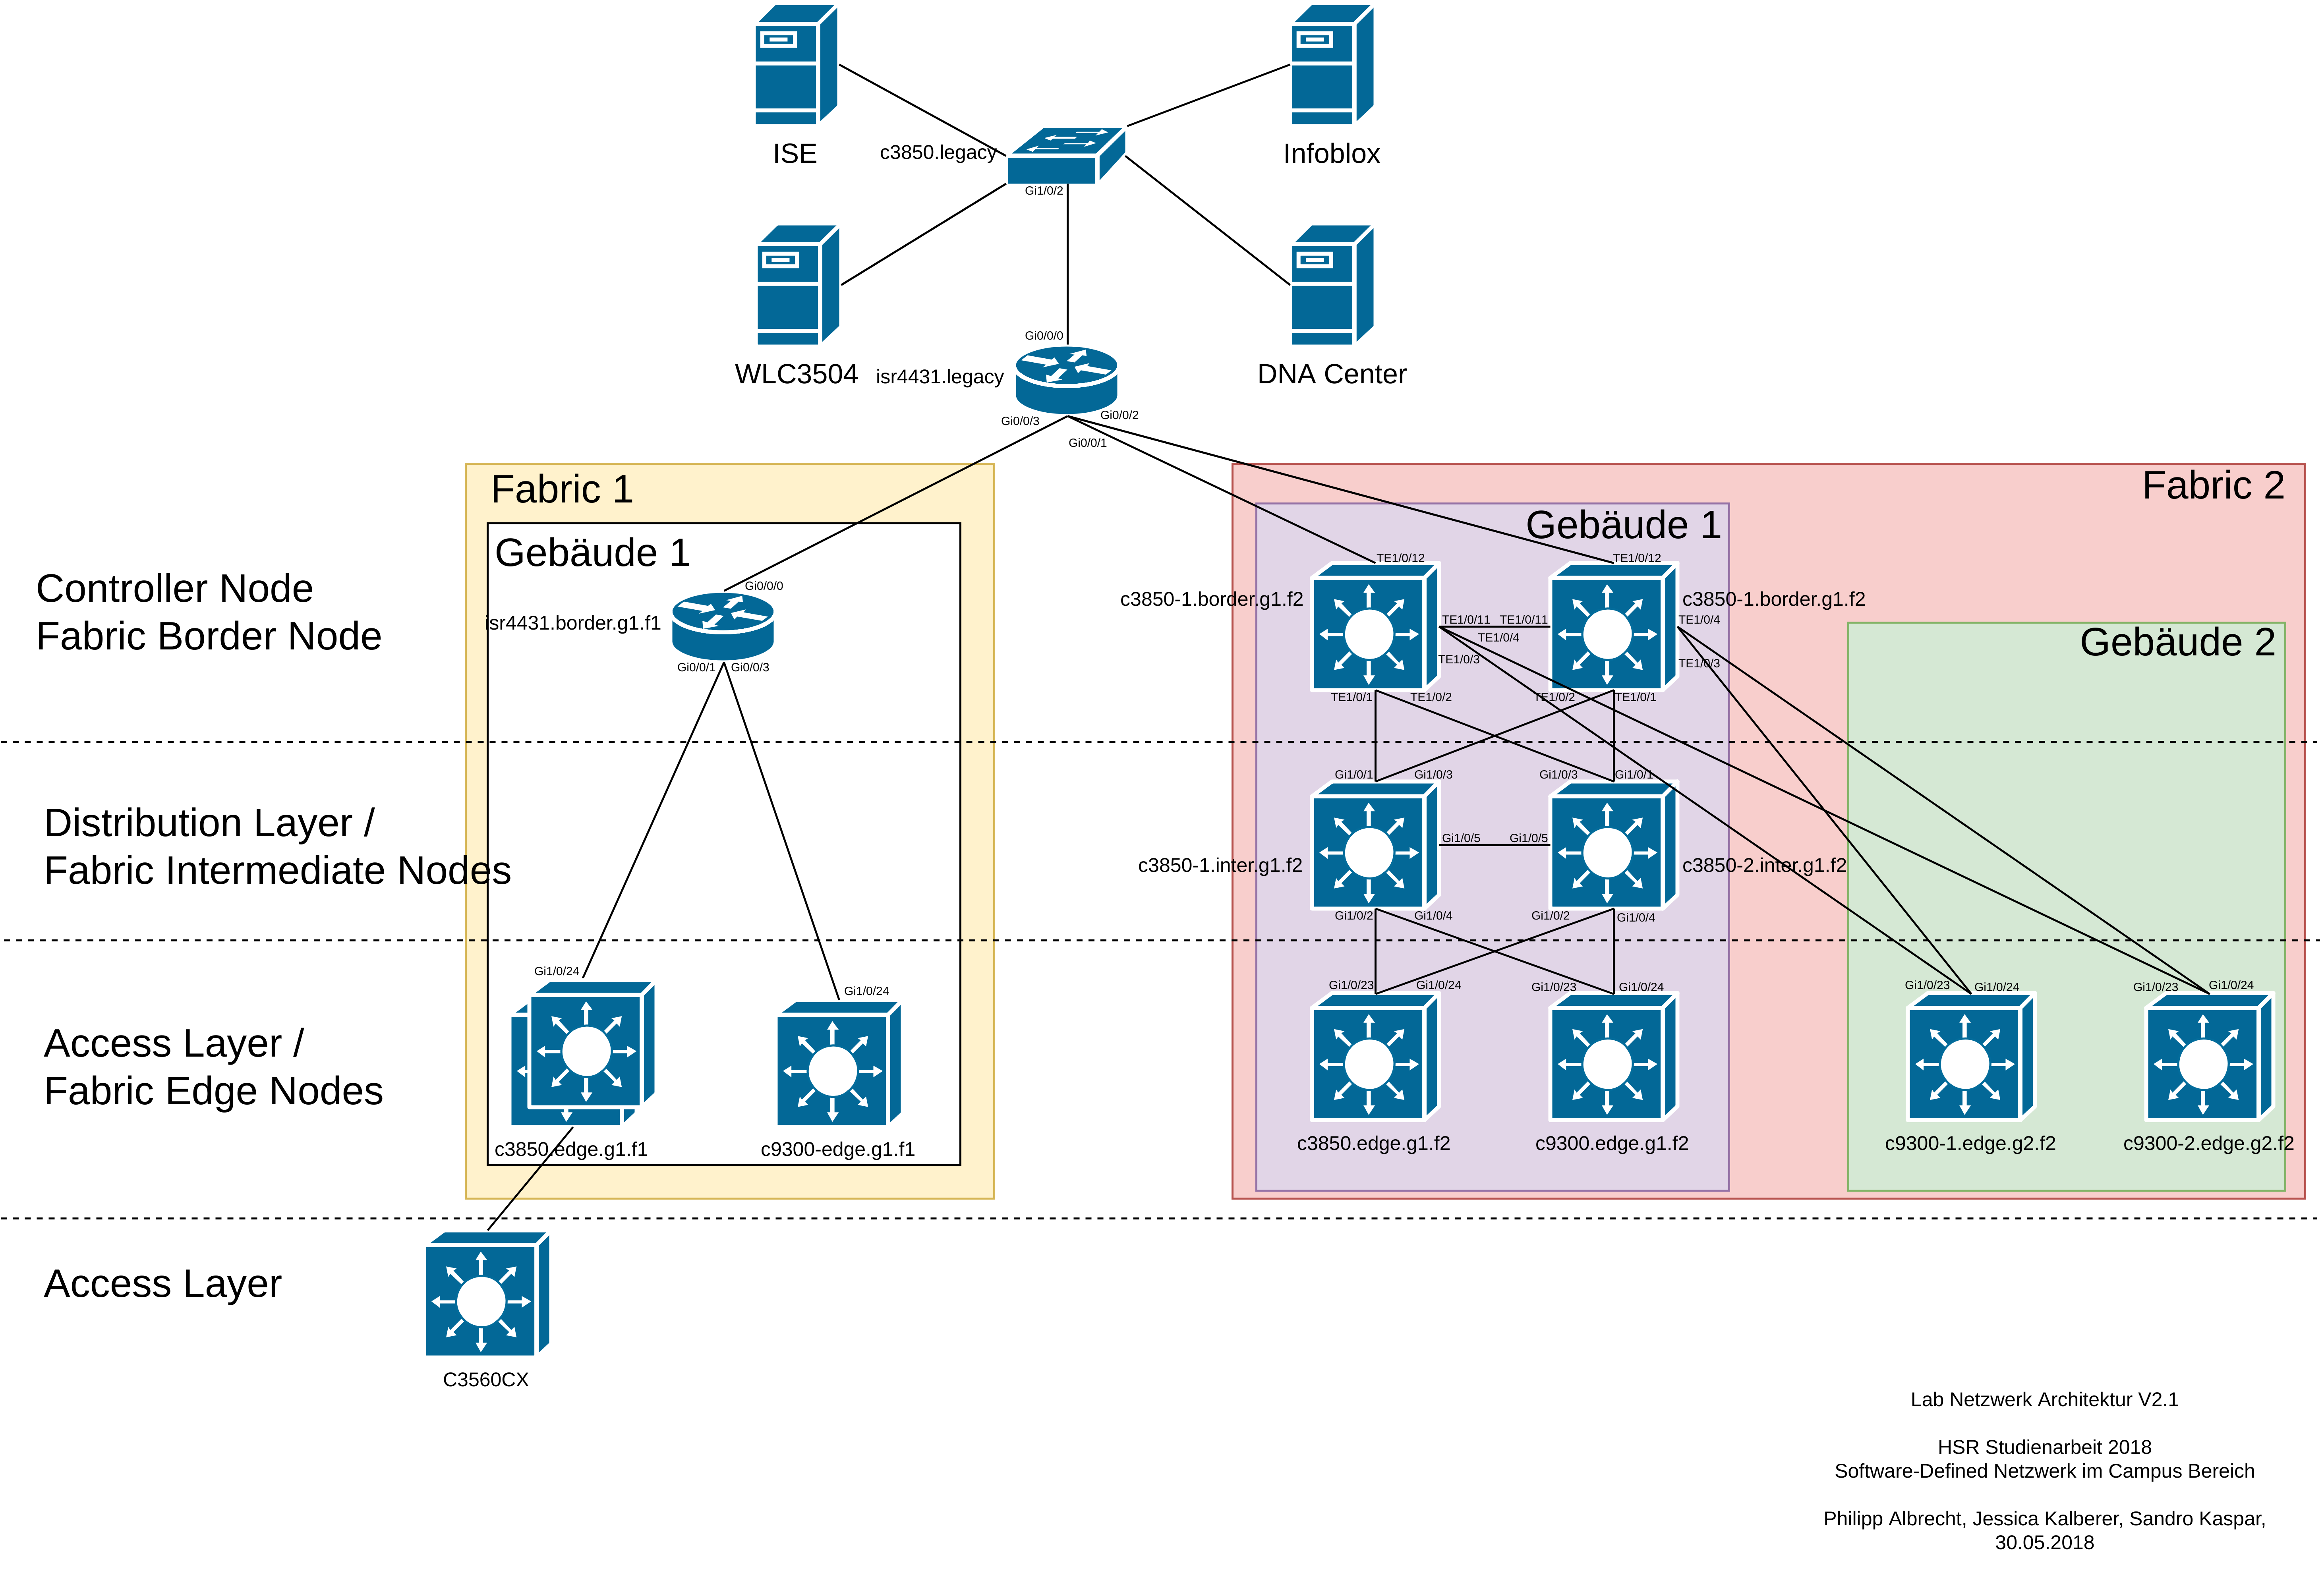
\includegraphics[angle=90,width=0.9\linewidth]{img/LabNetworkArchitecture-Interfaces.png}\\[1px]
	\caption{Lab Architecture with physical Interfaces}
	\label{fig:Lab Architecture with physical Interfaces}
\end{figure}


\subsection{Netzwerkarchitekturen Vergleich}
Hauptunterschiede zwischen der klassischen Netzwerkarchitektur und der "Modernen" Software-Defined Access Architektur. 

\begin{itemize}
	\item Bis zur Fabric Edge Nodes (Vergleichbar mit dem Access Layer) unterliegt ein L3 Netzwerk. 
	\item Kein Einsatz von Spanning Tree Protocol (STP) oder Virtual Switching Systems (VSS) auf Distribution Layer notwendig, da das Underlay Netzwerk rein L3 ist und Routing Protokolle (BGP oder Open Shortest Path First (OSPF)) zum Einsatz kommen.
	\item Der Distribution Layer nimmt neu als Fabric Intermediate Nodes nur noch die Funktion als L3 Brücke beziehungsweise VXLAN Transporteur ein, anstatt die Grenze zwischen L3 und L2 zu sein. Die Fabric Intermediate Nodes sind optional. 
	\item Während beim klassischen Design die logische Netzwerkarchitektur direkt Abhängig ist von der physikalischen Architektur, wird bei SDN die physikalische Netzwerkarchitektur von der logischen Architektur getrennt. Dabei wird von der Physical Fabric Topology oder auch dem Underlay und den entsprechenden L2 und L3 Overlay Network gesprochen. 
\end{itemize}

\begin{figure}[H]
	\centering
	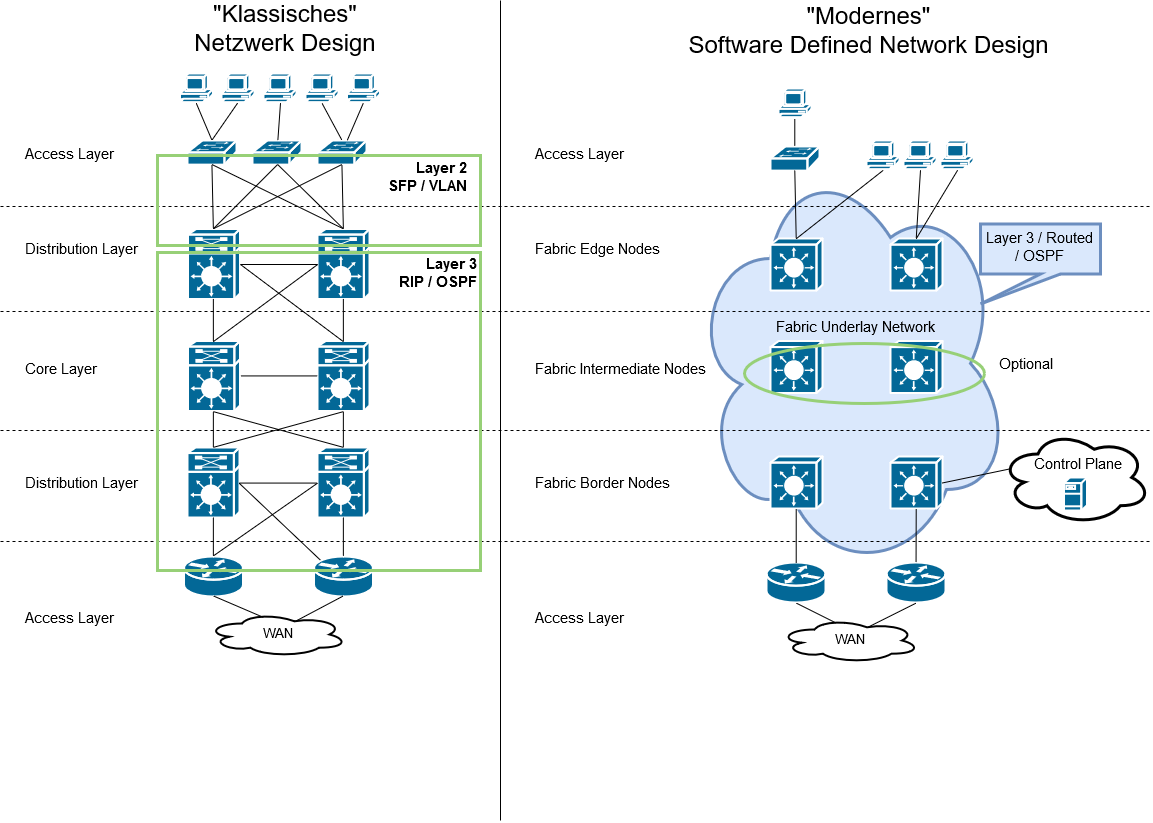
\includegraphics[width=1\linewidth]{img/LabNetworkArchitecture_Vergleich.png}\\[1px]
	\caption{Netzwerk Architektur Vergleich}
	\label{fig:LabNetworkArchitectureVergleich}
\end{figure}


\subsection{Maximale Skalierungen}
Nachfolgend werden die aktuell maximalen Skalierungen des DNA Centers, sowie der Border und Edge Nodes aufgelistet. Diese Skalierungen sind vor allem in einer ersten Evaluationsphase von Bedeutung, um zu entscheiden ob die Produkte mit den aktuellen maximalen Skalierungen überhaupt in Betracht gezogen werden können. 
\begin{figure}[H]
	\centering
	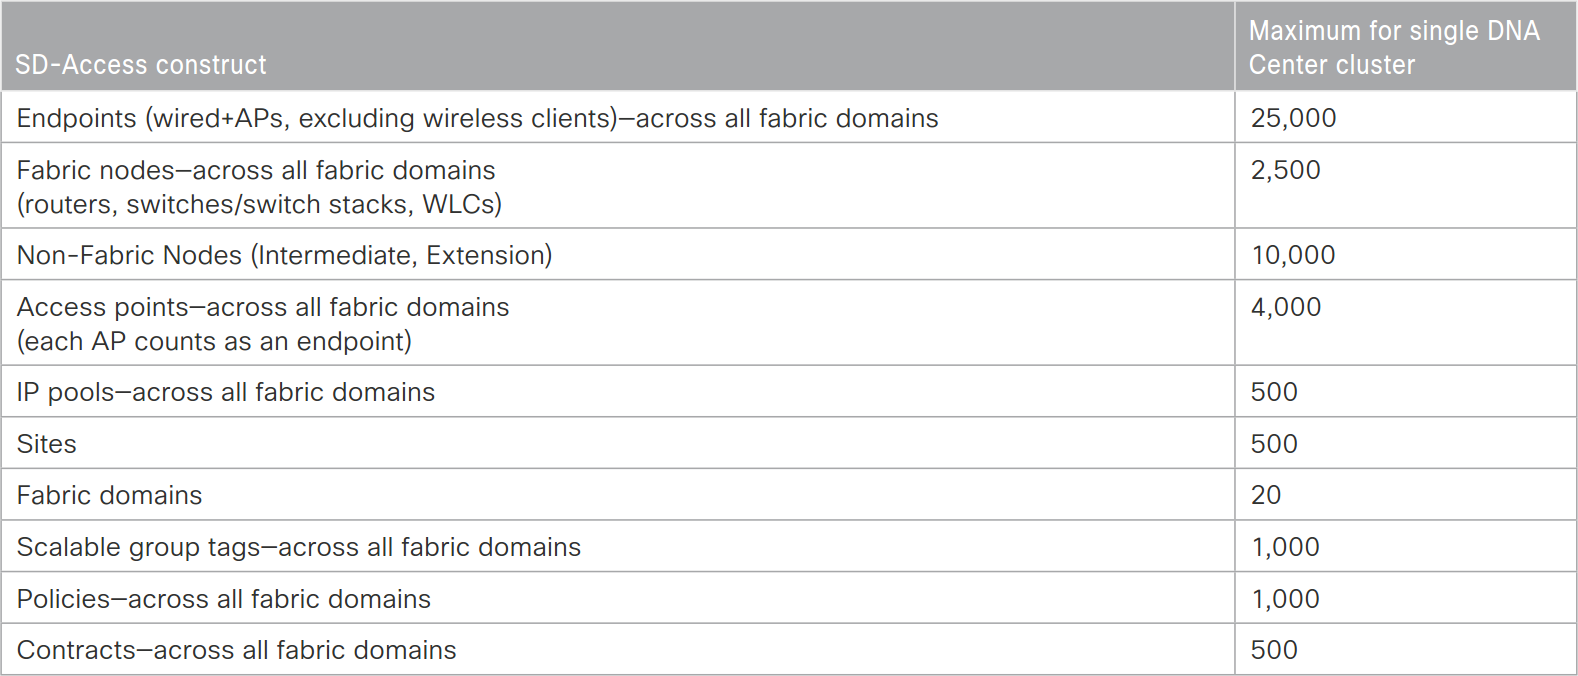
\includegraphics[width=1\linewidth]{img/MaximumScale-HACluster.png}\\[1px]
	\caption{DNA Center Maximum Scale Constraints HA Cluster \cite{sda-designguide}}
	\label{fig:Maximum Scale HACluster}
\end{figure}


\begin{figure}[H]
	\centering
	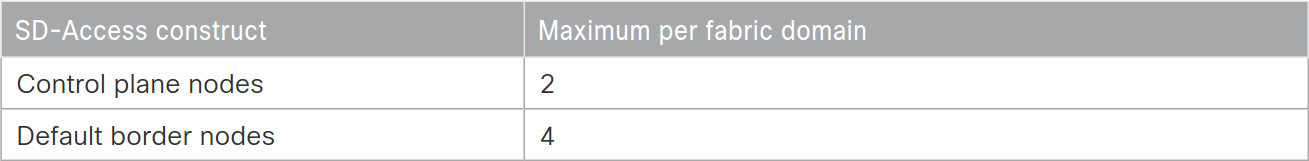
\includegraphics[width=1\linewidth]{img/MaximumScale-Fabric.png}\\[1px]
	\caption{DNA Center Maximum Scale Constraints Fabric \cite{sda-designguide}}
	\label{fig:Maximum Scale Fabric}
\end{figure}

\begin{figure}[H]
	\centering
	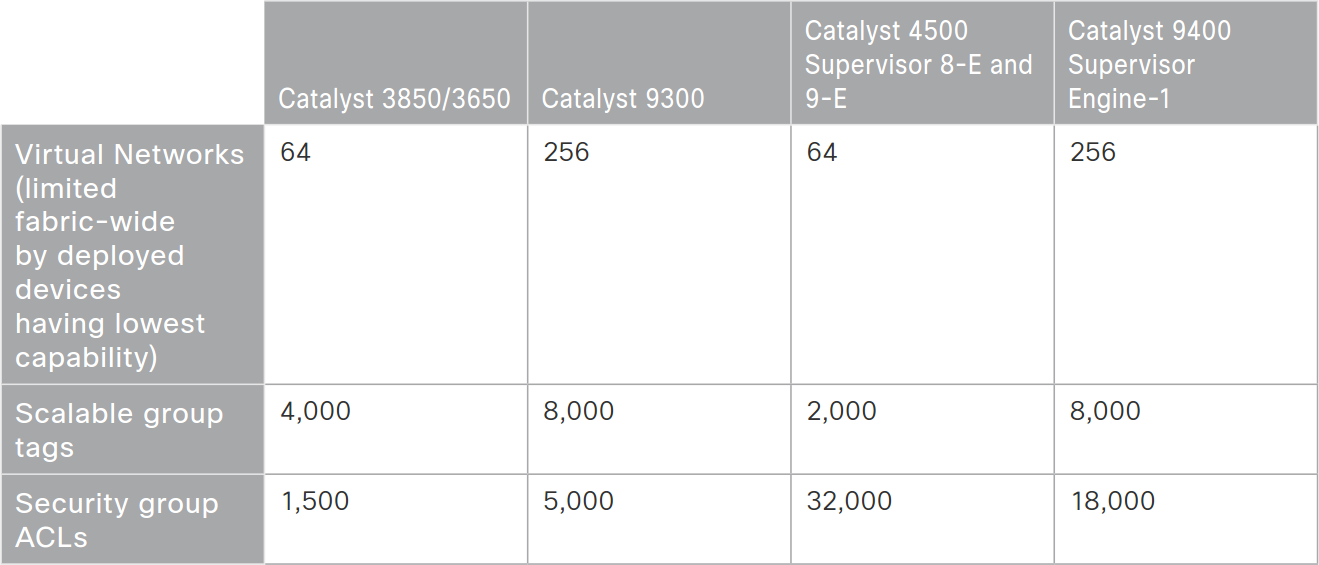
\includegraphics[width=1\linewidth]{img/MaximumScale-EdgeNode.png}\\[1px]
	\caption{SDA Edge Node Scale Constraints \cite{sda-designguide}}
	\label{fig:SDA Edge Node Scale Constraints}
\end{figure}

\begin{figure}[H]
	\centering
	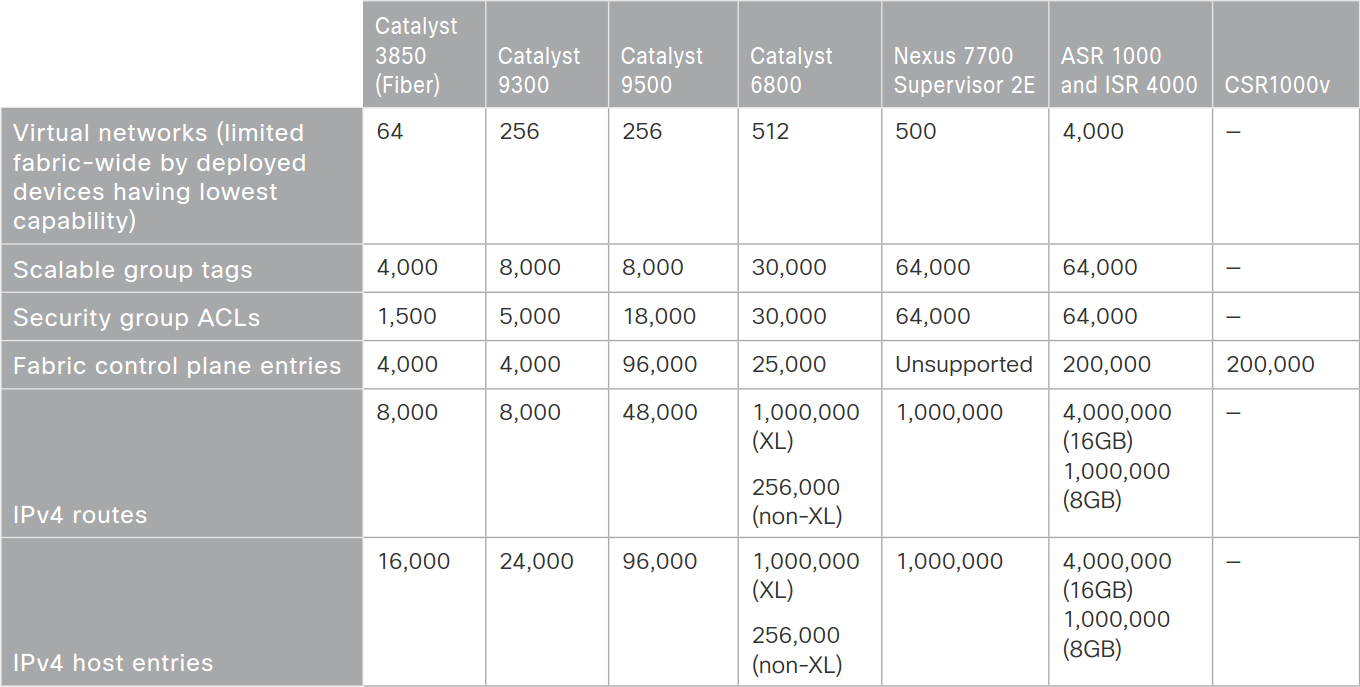
\includegraphics[width=1\linewidth]{img/MaximumScale-BorderNode.png}\\[1px]
	\caption{SDA Border Node Scale Constraints \cite{sda-designguide}}
	\label{fig:SDA Border Node Scale Constraints}
\end{figure}

\subsection{Anwendung und Vorgehen}
Bei der Architektur und Planung der Konfiguration wurden die vorgegebenen maximalen Skalierungen berücksichtigt. Es ist aber wichtig zu erwähnen, dass sich diese maximalen Skalierungen in jedem neuen Release des DNA Centers wieder ändern können.

Im nächsten Kapitel wird der genaue Vorgang der Installation, sowie auch der Konfiguration des DNA Centers und des Campus Netzwerkes erläutert (Siehe: Kapitel \ref{versuch1} Vorgang 1 und Kapitel \ref{versuch2} Vorgang 2)

